\documentclass[
  bibliography=totoc,     % Literatur im Inhaltsverzeichnis
  captions=tableheading,  % Tabellenüberschriften
  titlepage=firstiscover, % Titelseite ist Deckblatt
]{scrartcl}

% Paket float verbessern
\usepackage{scrhack}

% Warnung, falls nochmal kompiliert werden muss
\usepackage[aux]{rerunfilecheck}

% unverzichtbare Mathe-Befehle
\usepackage{amsmath}
% viele Mathe-Symbole
\usepackage{amssymb}
% Erweiterungen für amsmath
\usepackage{mathtools}

% Fonteinstellungen
\usepackage{fontspec}
% Latin Modern Fonts werden automatisch geladen
% Alternativ:
%\setromanfont{Libertinus Serif}
%\setsansfont{Libertinus Sans}
%\setmonofont{Libertinus Mono}
\recalctypearea % Wenn man andere Schriftarten gesetzt hat,
% sollte man das Seiten-Layout neu berechnen lassen

% deutsche Spracheinstellungen
\usepackage{polyglossia}
\setmainlanguage{german}


\usepackage[
  math-style=ISO,    % ┐
  bold-style=ISO,    % │
  sans-style=italic, % │ ISO-Standard folgen
  nabla=upright,     % │
  partial=upright,   % ┘
  warnings-off={           % ┐
    mathtools-colon,       % │ unnötige Warnungen ausschalten
    mathtools-overbracket, % │
},                       % ┘
]{unicode-math}

% traditionelle Fonts für Mathematik
\setmathfont{Latin Modern Math}
% Alternativ:
%\setmathfont{Libertinus Math}

\setmathfont{XITS Math}[range={scr, bfscr}]
\setmathfont{XITS Math}[range={cal, bfcal}, StylisticSet=1]

% Zahlen und Einheiten
\usepackage[
locale=DE,                   % deutsche Einstellungen
separate-uncertainty=true,   % immer Fehler mit \pm
per-mode=symbol-or-fraction, % / in inline math, fraction in display math
]{siunitx}

% chemische Formeln
\usepackage[
version=4,
math-greek=default, % ┐ mit unicode-math zusammenarbeiten
text-greek=default, % ┘
]{mhchem}

% richtige Anführungszeichen
\usepackage[autostyle]{csquotes}

% schöne Brüche im Text
\usepackage{xfrac}

% Standardplatzierung für Floats einstellen
\usepackage{float}
\floatplacement{figure}{htbp}
\floatplacement{table}{htbp}

% Floats innerhalb einer Section halten
\usepackage[
section, % Floats innerhalb der Section halten
below,   % unterhalb der Section aber auf der selben Seite ist ok
]{placeins}

% Seite drehen für breite Tabellen: landscape Umgebung
\usepackage{pdflscape}

% Captions schöner machen.
\usepackage[
  labelfont=bf,        % Tabelle x: Abbildung y: ist jetzt fett
  font=small,          % Schrift etwas kleiner als Dokument
  width=0.9\textwidth, % maximale Breite einer Caption schmaler
]{caption}
% subfigure, subtable, subref
\usepackage{subcaption}

% Grafiken können eingebunden werden
\usepackage{graphicx}
% größere Variation von Dateinamen möglich
\usepackage{grffile}

% schöne Tabellen
\usepackage{booktabs}

% Verbesserungen am Schriftbild
\usepackage{microtype}

% Literaturverzeichnis
\usepackage[style=alphabetic,]{biblatex}
% Quellendatenbank
\addbibresource{lit.bib}
\addbibresource{programme.bib}

% Hyperlinks im Dokument
\usepackage[
  unicode,        % Unicode in PDF-Attributen erlauben
  pdfusetitle,    % Titel, Autoren und Datum als PDF-Attribute
  pdfcreator={},  % ┐ PDF-Attribute säubern
  pdfproducer={}, % ┘
]{hyperref}
% erweiterte Bookmarks im PDF
\usepackage{bookmark}

% Trennung von Wörtern mit Strichen
\usepackage[shortcuts]{extdash}

\title{V47: Molwärme von Kupfer}
\author{
  Simon Schulte
  \texorpdfstring{
    \\
    \href{mailto:simon.schulte@udo.edu}{simon.schulte@udo.edu}
  }{}
  \texorpdfstring{\and}{, }
  Tim Sedlaczek
  \texorpdfstring{
    \\
    \href{mailto:tim.sedlaczek@udo.edu}{tim.sedlaczek@udo.edu}
  }{}
}
\publishers{TU Dortmund – Fakultät Physik}

\date{Durchführung: 23.04.2018\\
      Abgabe: 27.04.2018}


\begin{document}

\maketitle
\thispagestyle{empty}
\setcounter{page}{1}
\pagenumbering{arabic}
\section{Theorie}
\label{sec:theorie}
Ziel des Versuchs ist die Untersuchung der Temperaturabhängigkeit der
Molwärme $C_{\mathrm{V}}$ von Kupfer, sowie die Bestimmung der
materialspezifischen Größe~$\theta_{\mathrm{D}}$. Dazu wird die Molwärme bei
verschiedenen Temperaturen gemessen und mit der Theorie verglichen. Dabei ergeben
sich drei verschiedene theoretische Modelle.
\subsection{Die klassische Theorie der Molwärme}
Betrachtet man das System des Festkörpers innerhalb der klassischen Physik, so
verteilt sich die Wärmenergie, die einem Festkörper zugeführt wird, gleichmäßig auf
alle drei Freiheitsgrade des Atoms. Pro
Freiheitsgrad besitzt jedes Atom im Mittel die
Energie $\frac{1}{2}k_{\mathrm{B}}T$, sodass sich für alle Feiheitsgrade und
die beiden Energieformen eine mittlere Energie von
%
\begin{equation}
   \langle E \rangle =2\cdot 3\cdot\frac{1}{2}k_{\mathrm{B}}T
\end{equation}
%
pro Atom ergibt. Dabei ist $k_{\mathrm{B}}$ die Bolzmann-Konstante und $T$ die
Temperatur. Für ein Mol an Atomen im Festkörper ergibt
sich über die passende thermodynamische Relation die material- und
temperaturunabhängige Größe $C$ zu:
%
\begin{equation}
  C_{\mathrm{V}}=\left(\frac{\partial}{\partial T}U\cdot N_{\mathrm{L}}\right)_{\mathrm{V}}=3R
  \label{eq:CV}
\end{equation}
%
Experimentelle Erfahrungen zeigen allerdings sehr wohl eine Material- und
Temperaturabhängigkeit. Der Wert $3R$ gilt nur für sehr hohe Temperaturen als
gute Näherung.
%
\subsection{Die Theorie nach Einstein}
%
Das Modell nach Einstein berücksichtigt die Quantelung der Schwingungsenergie. So
wird hier angenommen, dass Energie zwischen den einzelnen Atomen im Festkörper
nur in Vielfachen von~$\hbar\omega$ ausgetauscht werden kann. $\omega$ ist dabei
die als einheitlich angenommene bei den Schwingern im Kristall vorliegende
Frequenz. Die Wahrscheinlichkeit, dass nun ein Oszillator bei gegebener
Temperatur~$T$ im Gleichgewicht mit der Umgebung die Energie~$n\hbar\omega$
besitzt, folgt dabei der Boltzmann-Verteilung:
%
\begin{equation}
  W(n)=e^{-\frac{n\hbar\omega}{k_{\mathrm{B}}T}}.
\end{equation}
%
Die Summation über alle Energien gewichtet mit ihrer Wahrscheinlichkeit ergibt
eine mittlere Energie pro Atom von:
%
\begin{equation}
  U_{\text{Einstein}}=\frac{\hbar\omega}{e^{\sfrac{\hbar\omega}{k_{\mathrm{B}}T}}-1}.
\end{equation}
%
Diese liegt unterhalb der klassisch vorhergesagten Energie. Damit ergibt sich
für die Molwärme:
%
\begin{equation}
  C_{\mathrm{V}}=3R\frac{1}{T^2}\frac{\hbar^2\omega^2}{k_{\mathrm{B}}^2}\frac{e^{\frac{\hbar\omega}{k_{\mathrm{B}}T}}}{(e^{\frac{\hbar\omega}{k_{\mathrm{B}}T}}-1)^2}.
\end{equation}
Allerdings weicht vor allem der Verlauf im Bereich tiefer Temperaturen stark ab
vom Verlauf der experimentellen Kurve.
\subsection{Die Theorie nach Debye}
Die Abweichung der Einsteintheorie im Bereich tiefer Temperaturen lässt sich
dadurch erklären, dass dort von einer singulären Frequenz ausgegangen wird.
Das Modell nach Debye berücksichtigt nun, dass die Frequenzen der
Eigenschwingungen der Atome im Festkörper nicht mehr einheitlich sind, sondern
nach einer sogenannten Spektralverteilung~$Z(\omega)$ verteilt sind.  Das Modell
berücksichtigt allerdings nicht die Frequenz- sowie die Richtungsabhängigkeit der
Phasengeschwindigkeit einer elastischen Welle im Kristall und die Rolle der
Leitungselektronen, welche allerdings erst bei sehr niedrigen Temperaturen
nennenswert wird. Ein Kristall von endlichen Ausmessungen aus~$N_{\mathrm{L}}$
Atomen besitzt nur $3N_{\mathrm{L}}$ viele verschiedene Schwingungsfrequenzen.
Daher muss das Integral über die
Spektralverteilung auf diesen Wert konvergieren. Dies ist nur möglich, wenn es
eine endliche Grenzfrequenz $\omega_{\mathrm{D}}$ gibt. Es gilt also:
%
\begin{equation}
  \int_0^{\omega_{\mathrm{D}}}Z(\omega)d\omega=3N_{\mathrm{L}}.
  \label{eq:konv}
\end{equation}
%
Aus
\begin{equation}
  \omega_D^3 = \frac{18 \pi² N_L}{L^3} \frac{1}{\frac{1}{{v_l}^3} + \frac{2}{{v_{tr}}^3}}
  \label{fürrune<3}
\end{equation}
folgt
\begin{equation*}
  Z(\omega) \symup d \omega = \frac{9N_L}{{\omega_D}^3} \, \omega^2 \symup d \omega
\end{equation*}
und daraus
\begin{equation}
  {C_V}_{\symup{De}} = 9 R \, \left(\frac{T}{\theta_D}\right)^3 \int_0^{\theta_D / T}
  \frac{x^4 \, \symup e^x}{(\symup e^x - 1)^2} \, \symup d x.
  \label{eqn:7}
\end{equation}
Dabei ist $\theta_D$ die Debye-Temperatur, welche materialabhängig ist. Aus \eqref{eqn:7}
wird ersichtlich, dass für die Grenzfälle kleiner und großer Temperaturen
\begin{align}
  \lim \limits_{T \to \infty}{{C_V}_{\symup{De}}} &= 3R \\
  \lim \limits_{T \to 0}{{C_V}_{\symup{De}}} &\propto T^3
\end{align}
gilt. Die $T^3$-Abhängigkeit beschreibt den Grenzfall kleiner Temperaturen besser
als das Einstein-Modell, ist aber aufgrund der getroffenen Annahme immer noch eine
Näherung. Auch die Leitungselektronen tragen zur Molwärme bei, allerdings ist ihr
Beitrag erst bei tiefen Temperaturen relevant und proportional zu $T$.


\section{Durchführung}
\label{sec:durchführung}
Der Versuchsaufbau ist in Abbildung~\ref{fig:aufbau} dargestellt. Die zu
untersuchende Kupferprobe befindet sich dabei in
einem Zylinder innerhalb des Rezipienten und ist von einem Dewar-Gefäß zur
Wärmeisolation umgeben. Damit verbunden sind die Pt-100 Widerstände zur
Temperaturmessung, sowie eine Heizwicklung für die Probe und eine für den
Kupferzylinder. Zur Vorbereitung der Messung wird zunächst der Rezipient über
das Ventil zur Vakuumpumpe evakuiert und mit Helium gefüllt. Helium dient dabei
als Medium für den Wärmeaustausch. Das gesamte Innere des Dewar-Gefäßes kann
dann durch Befüllen mit flüssigem Stickstoff auf etwa $\SI{80}{\kelvin}$
abgekühlt werden. Nachdem eine Abkühlung auf diesen Temperaturbereich erfolgt
ist, wird der Rezipient erneut evakuiert und mit der Messung begonnen.
Danach wird die Probe in \SI{7}{\celsius}-Schritten erwärmt. Es werden immer die benötigte
Zeitdauer, die Änderung der Temperatur des Zylinders und der Probe, die
Heizspannung und der Heizstrom aufgenommen. Um Wärmestrahlung zu vermeiden werden
außerdem der Zylinder und die Probe auf möglichst der gleichen Temperatur gehalten.
Es werden Werte bis ca. $\SI{300}{\kelvin}$ aufgenommen.

\begin{figure}
    \centering
    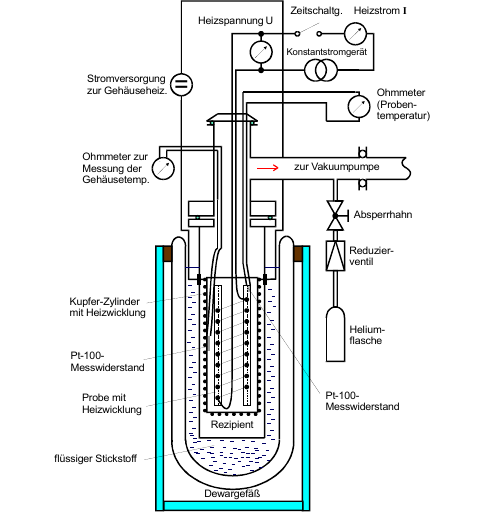
\includegraphics[width=\textwidth]{messapparatur.png}
    \caption{Schematischer Aufbau der verwendeten Messapparatur.\cite{V47}}
    \label{fig:aufbau}
\end{figure}

\end{document}
